
\subsection{Baseline method}
Our approach is based on the system proposed in \cite{ACCU:2015}.

\begin{figure*}[t]
\centering
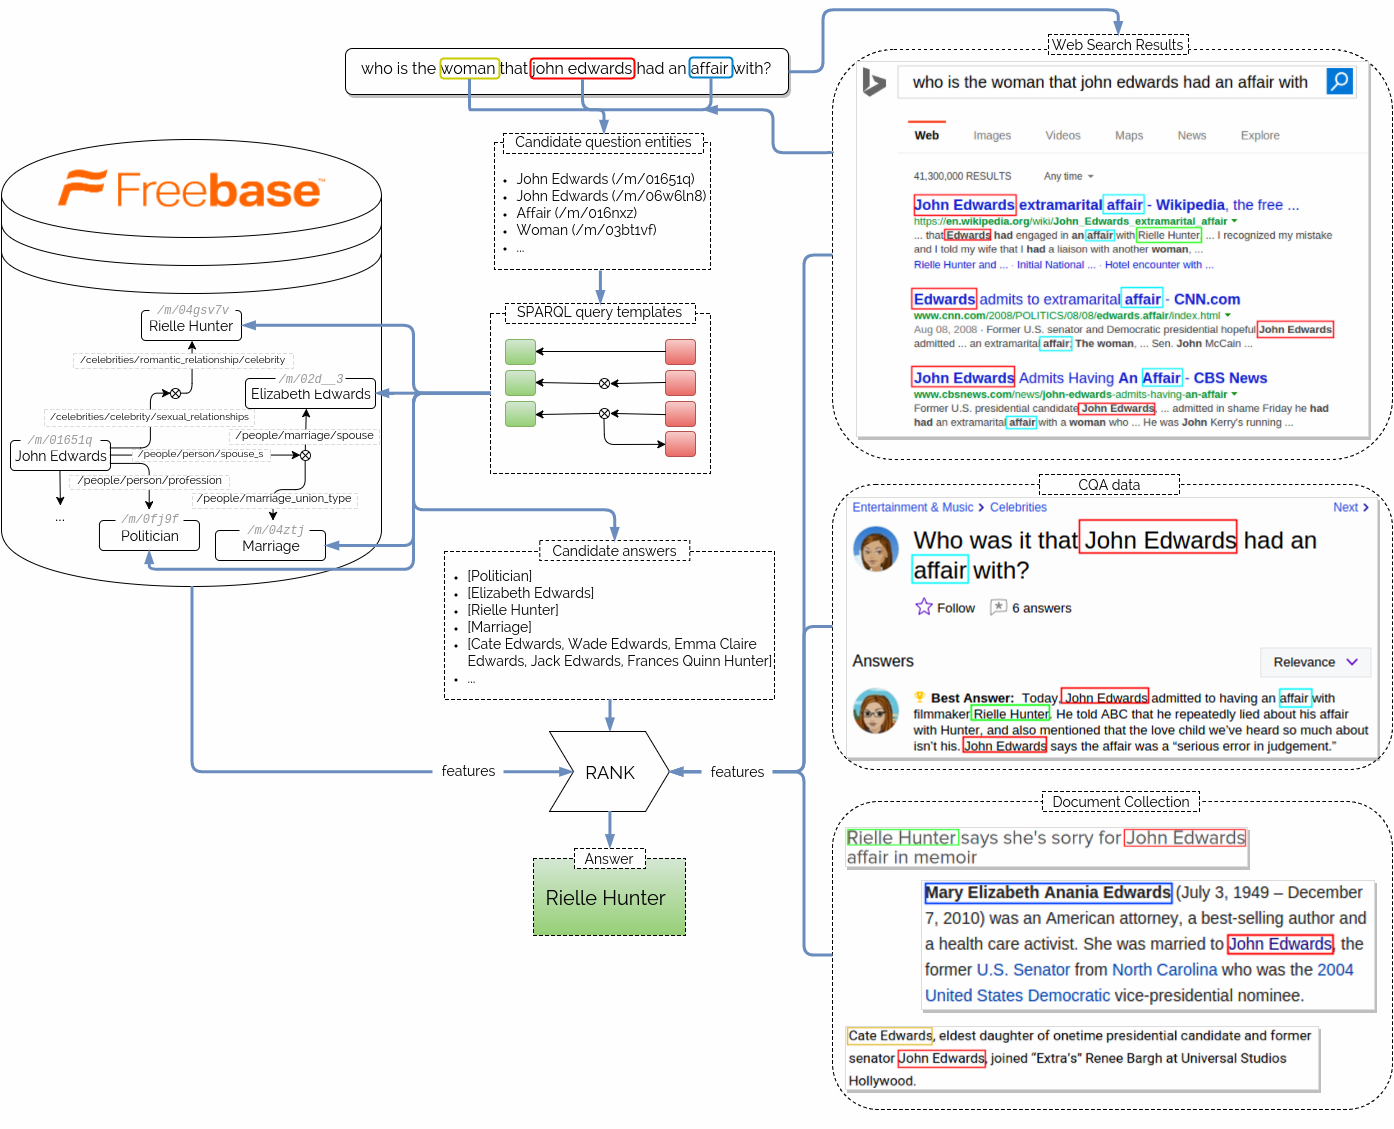
\includegraphics[width=\textwidth]{img/Text2KB_model}
\caption{The architecture of our Text2KB Question Answering system}
\label{fig:model}
\end{figure*}

\subsubsection{Extensions}
We implemented a couple of extensions of the baseline system.

\begin{itemize}
\item date range based filters
\item notable types based filters
\item notable types based model, used as a feature
\end{itemize}

\subsection{Unstructured data for KBQA}

\subsubsection{Text data in KB}
We use entity descriptions to generate a set of features for candidate answers.

\subsubsection{Web search results}
We issue question to a web search using Bing Web Search API\footnote{https://datamarket.azure.com/dataset/bing/search}.
Returned documents and snippets are used by our question answering system.

\begin{itemize}
\item Entity linking from snippets, similar to \cite{SMAPH_ERD:2014}.
\item Textual and entity similarity features based on search results documents and snippets
\end{itemize}

\subsubsection{Community Question Answering collection}
Using a collection of question-answer pairs from Yahoo! Answers we annotated questions and answers with entities and relations between pairs of entities.
This approach follows distant supervision approach for relation extraction \cite{savenkov-EtAl:2015:SRW}.
Pairs of question words and relations are used to generate features.

\subsubsection{Entity-linked collection of documents}
We take ClueWeb12 and use existing entity links generated by Google to build an index from entity pair to phrases, that occur around these entities in the collection.
This data is used to generate features for candidates.

\subsubsection{Wikipedia profile}
It would be nice to have Wikipedia pages for entities and use something like SDM score or something else as feature.